\documentclass[a4paper,11pt]{article}

\usepackage{geometry} % for making easy changes to page layout
\geometry{body={15cm,24cm}} % change height and width of main text


\usepackage{parskip} % for blank lines between paragraphs 

\usepackage{amsmath,amssymb} % for serious mathematics, such as \begin{align*} etc

\usepackage{graphicx} % for \includegraphics[width = 1\textwidth]{} etc
\usepackage{booktabs}

\title{GLM Practical}
\author{P806}
\date{7 Decembre 2022}

\begin{document}

\maketitle

\section{Introduction}

\section{Data Analysis}
For this section, note that the columns \texttt{private, freepoor, freerepat} are never all \texttt{1} for any sample. So, let's just create a variable \texttt{insurance} that is a categorical variable and has four different possible values: \texttt{private, freepoor, freerepat}, and \texttt{normal} 

\begin{figure}[h]
	\centering
	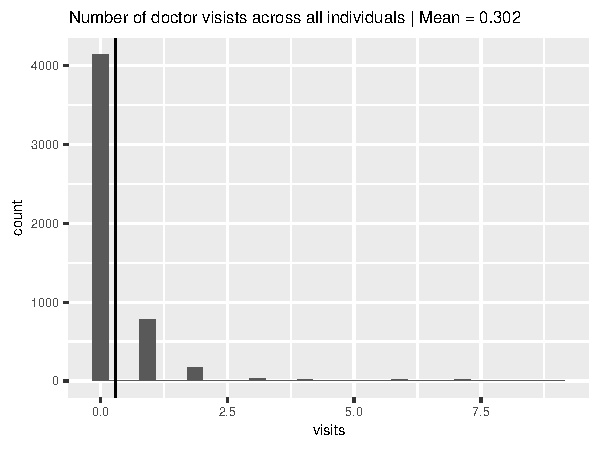
\includegraphics{../plots/histogram_of_visits.pdf}
	\caption{Histogram of entire dataset}
	\label{fig:hist_all}
\end{figure}

\begin{figure}[h]
	\centering
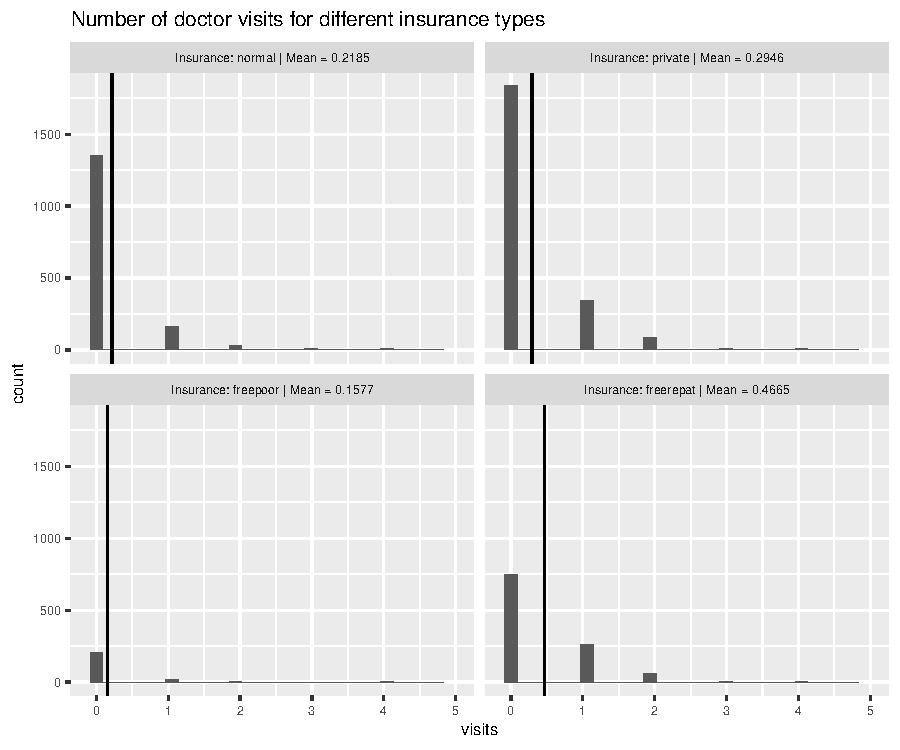
\includegraphics{../plots/histograms_of_insurances.pdf}
	\label{fig:hist_insurances}
		\caption{Histogram of data split by type of insurance}
\end{figure}

\begin{figure}[h]
	\centering
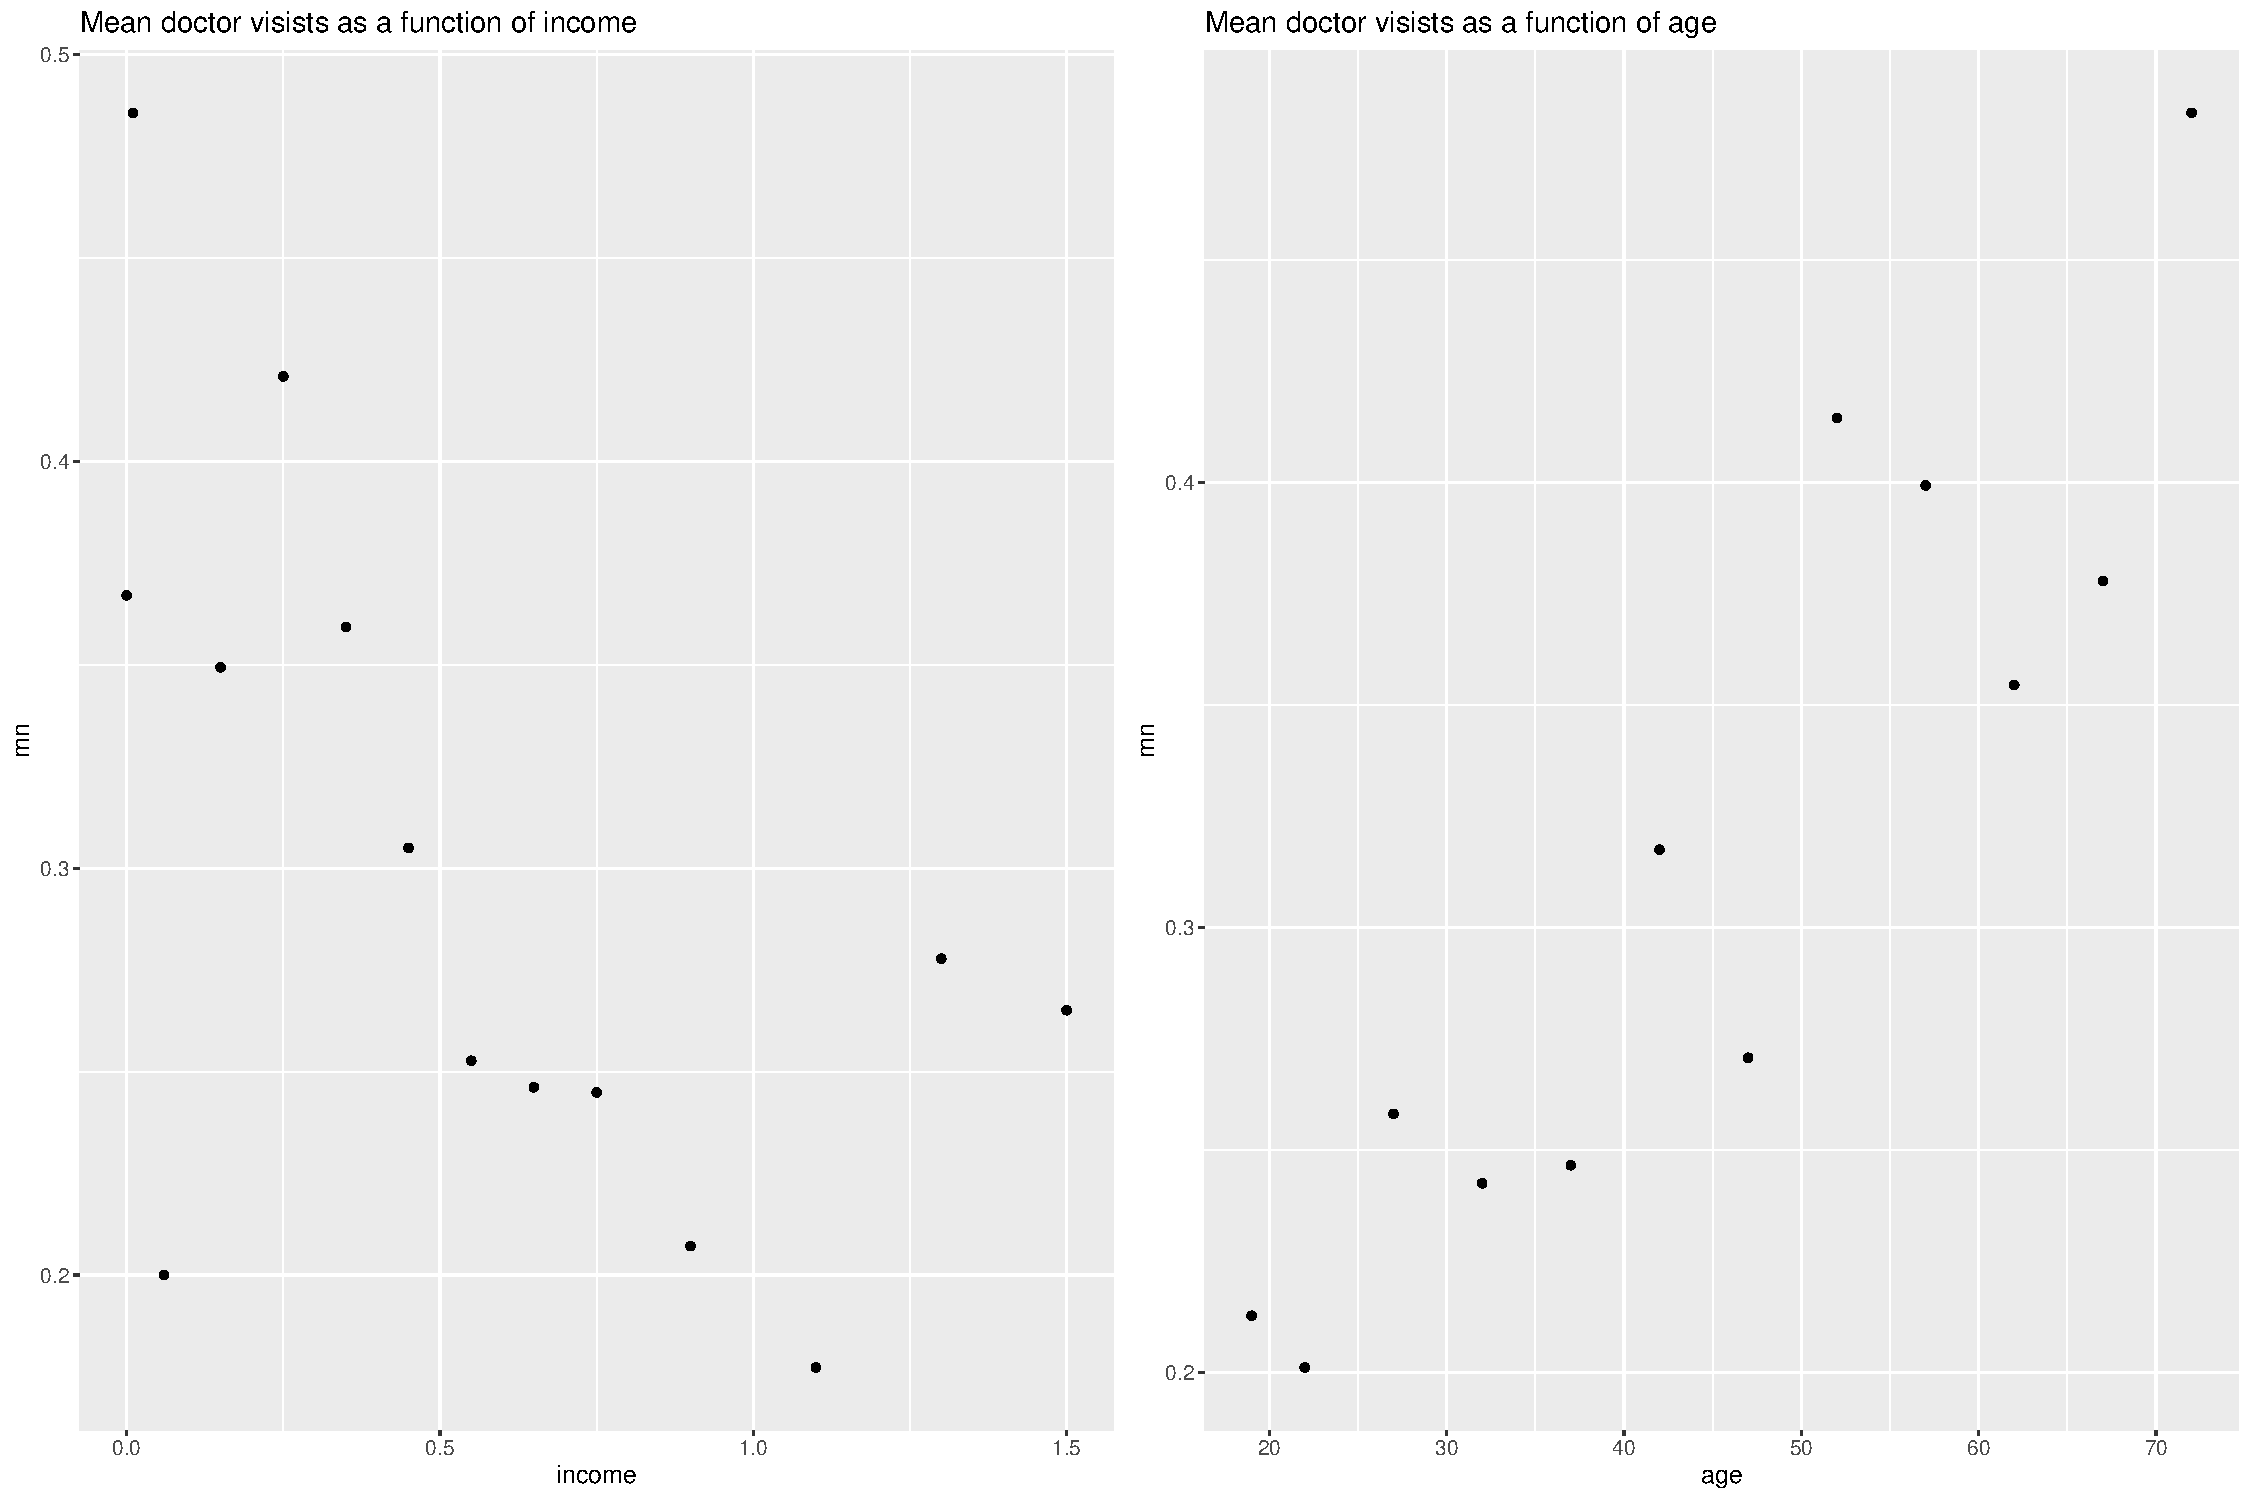
\includegraphics{../plots/mean_vs_income_and_age.pdf}
	\label{fig:scatter_income_and_age}
			\caption{Mean doctor visits as a function of income (left) and age (right)}
\end{figure}

\begin{figure}[h]
	\centering
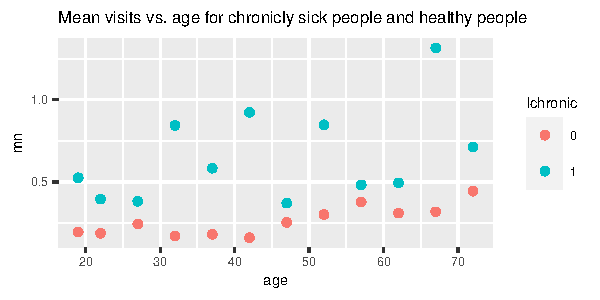
\includegraphics{../plots/mean_vs_age_and_chronic.pdf}
	\label{fig:scatter_age_and_chronic}
				\caption{Mean doctor visits as a function of age for responses of chronically ill and healthy people}
\end{figure}

\input{../report/descriptive_stats_fine.txt}
\input{../report/descriptive_stats_coarse.txt}

\end{document}
